\section{Theoretical background \& assumptions} \label{section: theoretical background}
\subsection{Assumptions}
in this project, we have developed a system to measure the forces applied to the front and rear of the foot during walking or running. We assumed that:
\begin{enumerate}
    \item the frequency of the force applied to the foot is about 1 Hz
    \item the maximum force applied to the sensor is about 1000 N
    \item the sensor has a white noise with a standard deviation of 0.001 V
    \item the urban electric noise frequency is about 50 Hz with a standard deviation of 0.1 V
\end{enumerate}
For a piezoelectric we have the following equation:
\begin{equation}
    V = \frac{dFt}{\epsilon_{0}\epsilon_{r}A}
\end{equation}
where :
\begin{itemize}
    \item $V$ is the voltage generated by the piezoelectric
    \item $d$ is the piezoelectric coefficient
    \item $F$ is the force applied to the piezoelectric
    \item $t$ is the thickness of the piezoelectric
    \item $\epsilon_{0}$ is the permittivity of free space
    \item $\epsilon_{r}$ is the relative permittivity of the piezoelectric
    \item $A$ is the area of the piezoelectric
\end{itemize}
We made the following assumptions:
\begin{itemize}
    \item $d = 2.89 \times 10^{-10} \frac{C}{N}$
    \item $t = 0.01 m$
    \item $\epsilon_{0} = 8.854 \times 10^{-12} \frac{F}{m}$
    \item $\epsilon_{r} = 1300$
    \item $A = 5^2 3.14 \times 10^{-4} m^{2}$
\end{itemize}
Thus in the case of the maximum force applied to the sensor, we have:
\begin{equation}
    V = \frac{2.89 \times 10^{-10} \times 1000 \times 0.01}{8.854 \times 10^{-12} \times 1300 \times 25 \times 3.14 \times 10^{-4}} = 3.2 V
\end{equation}
We assume that this voltage gets 1000 times weaker, so we have:
\begin{equation}
    V \simeq 0.0032 V
\end{equation}

If we assume that the input signal has a shape of sine wave, we have:
\begin{align}
     & V_{Front} = 0.032  sin(2\pi t)        \\
     & V_{Back} = 0.032  sin(2\pi t + \pi/2)
\end{align}

Where $V_{Front}$ is the voltage generated by the piezoelectric attached to the front of the foot and $V_{Back}$ is the voltage generated by the piezoelectric attached to the back of the foot.\\
The signal simulated in Matlab is shown below:
\begin{figure}[H]
    \centering
    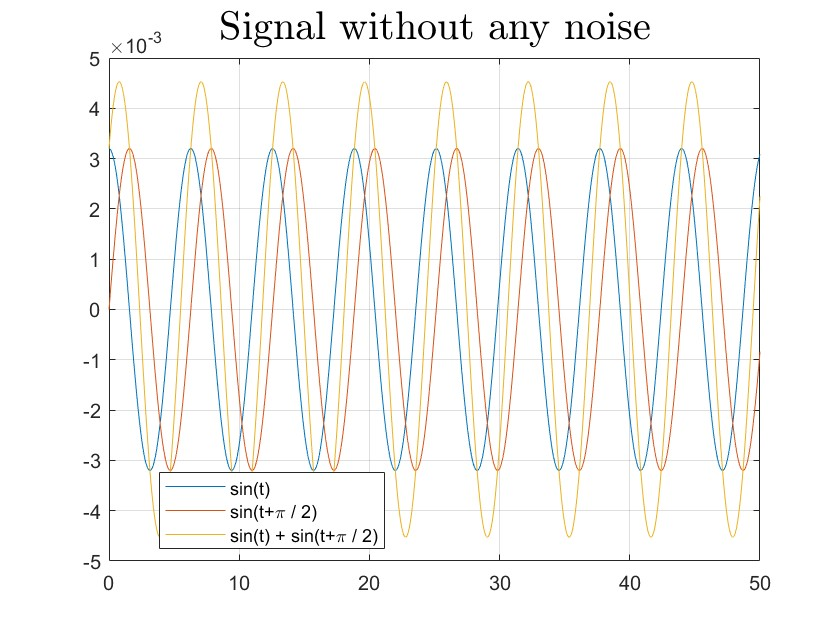
\includegraphics[width=0.8\textwidth]{../Report/Figures/2.CircuitDesign/InputSignal.jpg}
    \caption{The input signal whitout noise simulated in Matlab.}
\end{figure}
\subsection{Common circuits used to measure the force applied to the foot}
\subsubsection{Force plates}
The most common way to measure the force applied to the foot is using a force plate. A force plate is a device that measures the forces generated by a body standing on or moving across them. Force plates are used in a variety of settings including clinical, athletic, and industrial settings. Force plates are used to measure the ground reaction forces generated by a body standing on or moving across them, to quantify balance ability and assess gait and posture.
\\
\subsubsection{Pressure sensors}
Most common circuits used to measure the force applied have differential amplifiers. A differential amplifier is a type of electronic amplifier that amplifies the difference between two input voltages but suppresses any voltage common to the two inputs. It is an analog circuit with two inputs $V_{1}$ and $V_{2}$ and one output $V_{o}$ in which the output is ideally proportional to the difference between the two voltages $V_{1}$ and $V_{2}$. The gain of the amplifier is given by $A_{d} = \frac{V_{o}}{V_{1} - V_{2}}$.
\\
\subsubsection{Filters}
Then after ampflying the difference between the two voltages, we need to filter the noise. The most common filters used are low pass filters and high pass filters. A low-pass filter is a filter that passes signals with a frequency lower than a selected cutoff frequency and attenuates signals with frequencies higher than the cutoff frequency. The actual amount of attenuation for each frequency varies from filter to filter. A high-pass filter (HPF) is an electronic filter that passes signals with a frequency higher than a certain cutoff frequency and attenuates signals with frequencies lower than the cutoff frequency. The amount of attenuation for each frequency depends on the filter design.
\\
\subsection{Our circuit}
We deisgned a circuit containing two instrumentation amplifiers to measure the force applied to the sensor, then we have a differential amplifier to subtract the two signals and get the difference between the two forces applied to the front and rear of the foot. Then we have a low pass filter to filter the noise and get the original signal. Finally, we have a high pass filter to filter the 50 Hz noise and get the original signal.

\subsection{Theoretical background}
\subsubsection{Instrumentation amplifier}
An instrumentation amplifier is a type of differential amplifier that has been outfitted with input buffer amplifiers, which eliminate the need for input impedance matching and thus make the amplifier particularly suitable for use in measurement and test equipment. Additional characteristics include very low DC offset, low drift, low noise, very high open-loop gain, very high common-mode rejection ratio, and very high input impedances. Instrumentation amplifiers are used where great accuracy and stability of the circuit both short- and long-term are required.
\\
\subsubsection{Differential amplifier}
A differential amplifier is a type of electronic amplifier that amplifies the difference between two input voltages but suppresses any voltage common to the two inputs. It is an analog circuit with two inputs $V_{1}$ and $V_{2}$ and one output $V_{o}$ in which the output is ideally proportional to the difference between the two voltages $V_{1}$ and $V_{2}$. The gain of the amplifier is given by $A_{d} = \frac{V_{o}}{V_{1} - V_{2}}$.
\\
\subsubsection{Low pass filter}
A low-pass filter is a filter that passes signals with a frequency lower than a selected cutoff frequency and attenuates signals with frequencies higher than the cutoff frequency. The actual amount of attenuation for each frequency varies from filter to filter. A low-pass filter is the complement of a high-pass filter.
\\
\subsubsection{High pass filter}
A high-pass filter (HPF) is an electronic filter that passes signals with a frequency higher than a certain cutoff frequency and attenuates signals with frequencies lower than the cutoff frequency. The amount of attenuation for each frequency depends on the filter design. A high-pass filter is the complement of a low-pass filter.
\\
\subsubsection{Noise}
Noise is unwanted sound judged to be unpleasant, loud or disruptive to hearing. From a physics standpoint, noise is indistinguishable from sound, as both are vibrations through a medium, such as air or water. The difference arises when the brain receives and perceives a sound.
\\
\subsubsection{White noise}
White noise is a random signal having equal intensity at different frequencies, giving it a constant power spectral density. The term is used, with this or similar meanings, in many scientific and technical disciplines, including physics, acoustical engineering, telecommunications, statistical forecasting, and many more. White noise refers to a statistical model for signals and signal sources, rather than to any specific signal.
\\
\subsubsection{Urban electric noise}
Electric noise is the random fluctuations in an electrical signal, a characteristic of all electronic circuits. Noise generated by electronic devices varies greatly, as it can be produced by several different effects.
